% ============================================================
%  SUMMARY FIGURE — generated by generate_summary_figures.py
%  3 figures (B, dBdz, BgradB), each 5 rows × 2 cols,
%  shared axes, coord labels on right, column headers on top.
%
%  Required packages:
%    \usepackage{graphicx}
%    \usepackage{subfig}   (or just use \includegraphics directly)
%    \usepackage{caption}
% ============================================================

% ---------- Figure 1: B vs Position ----------
\begin{figure}[p]
    \centering
    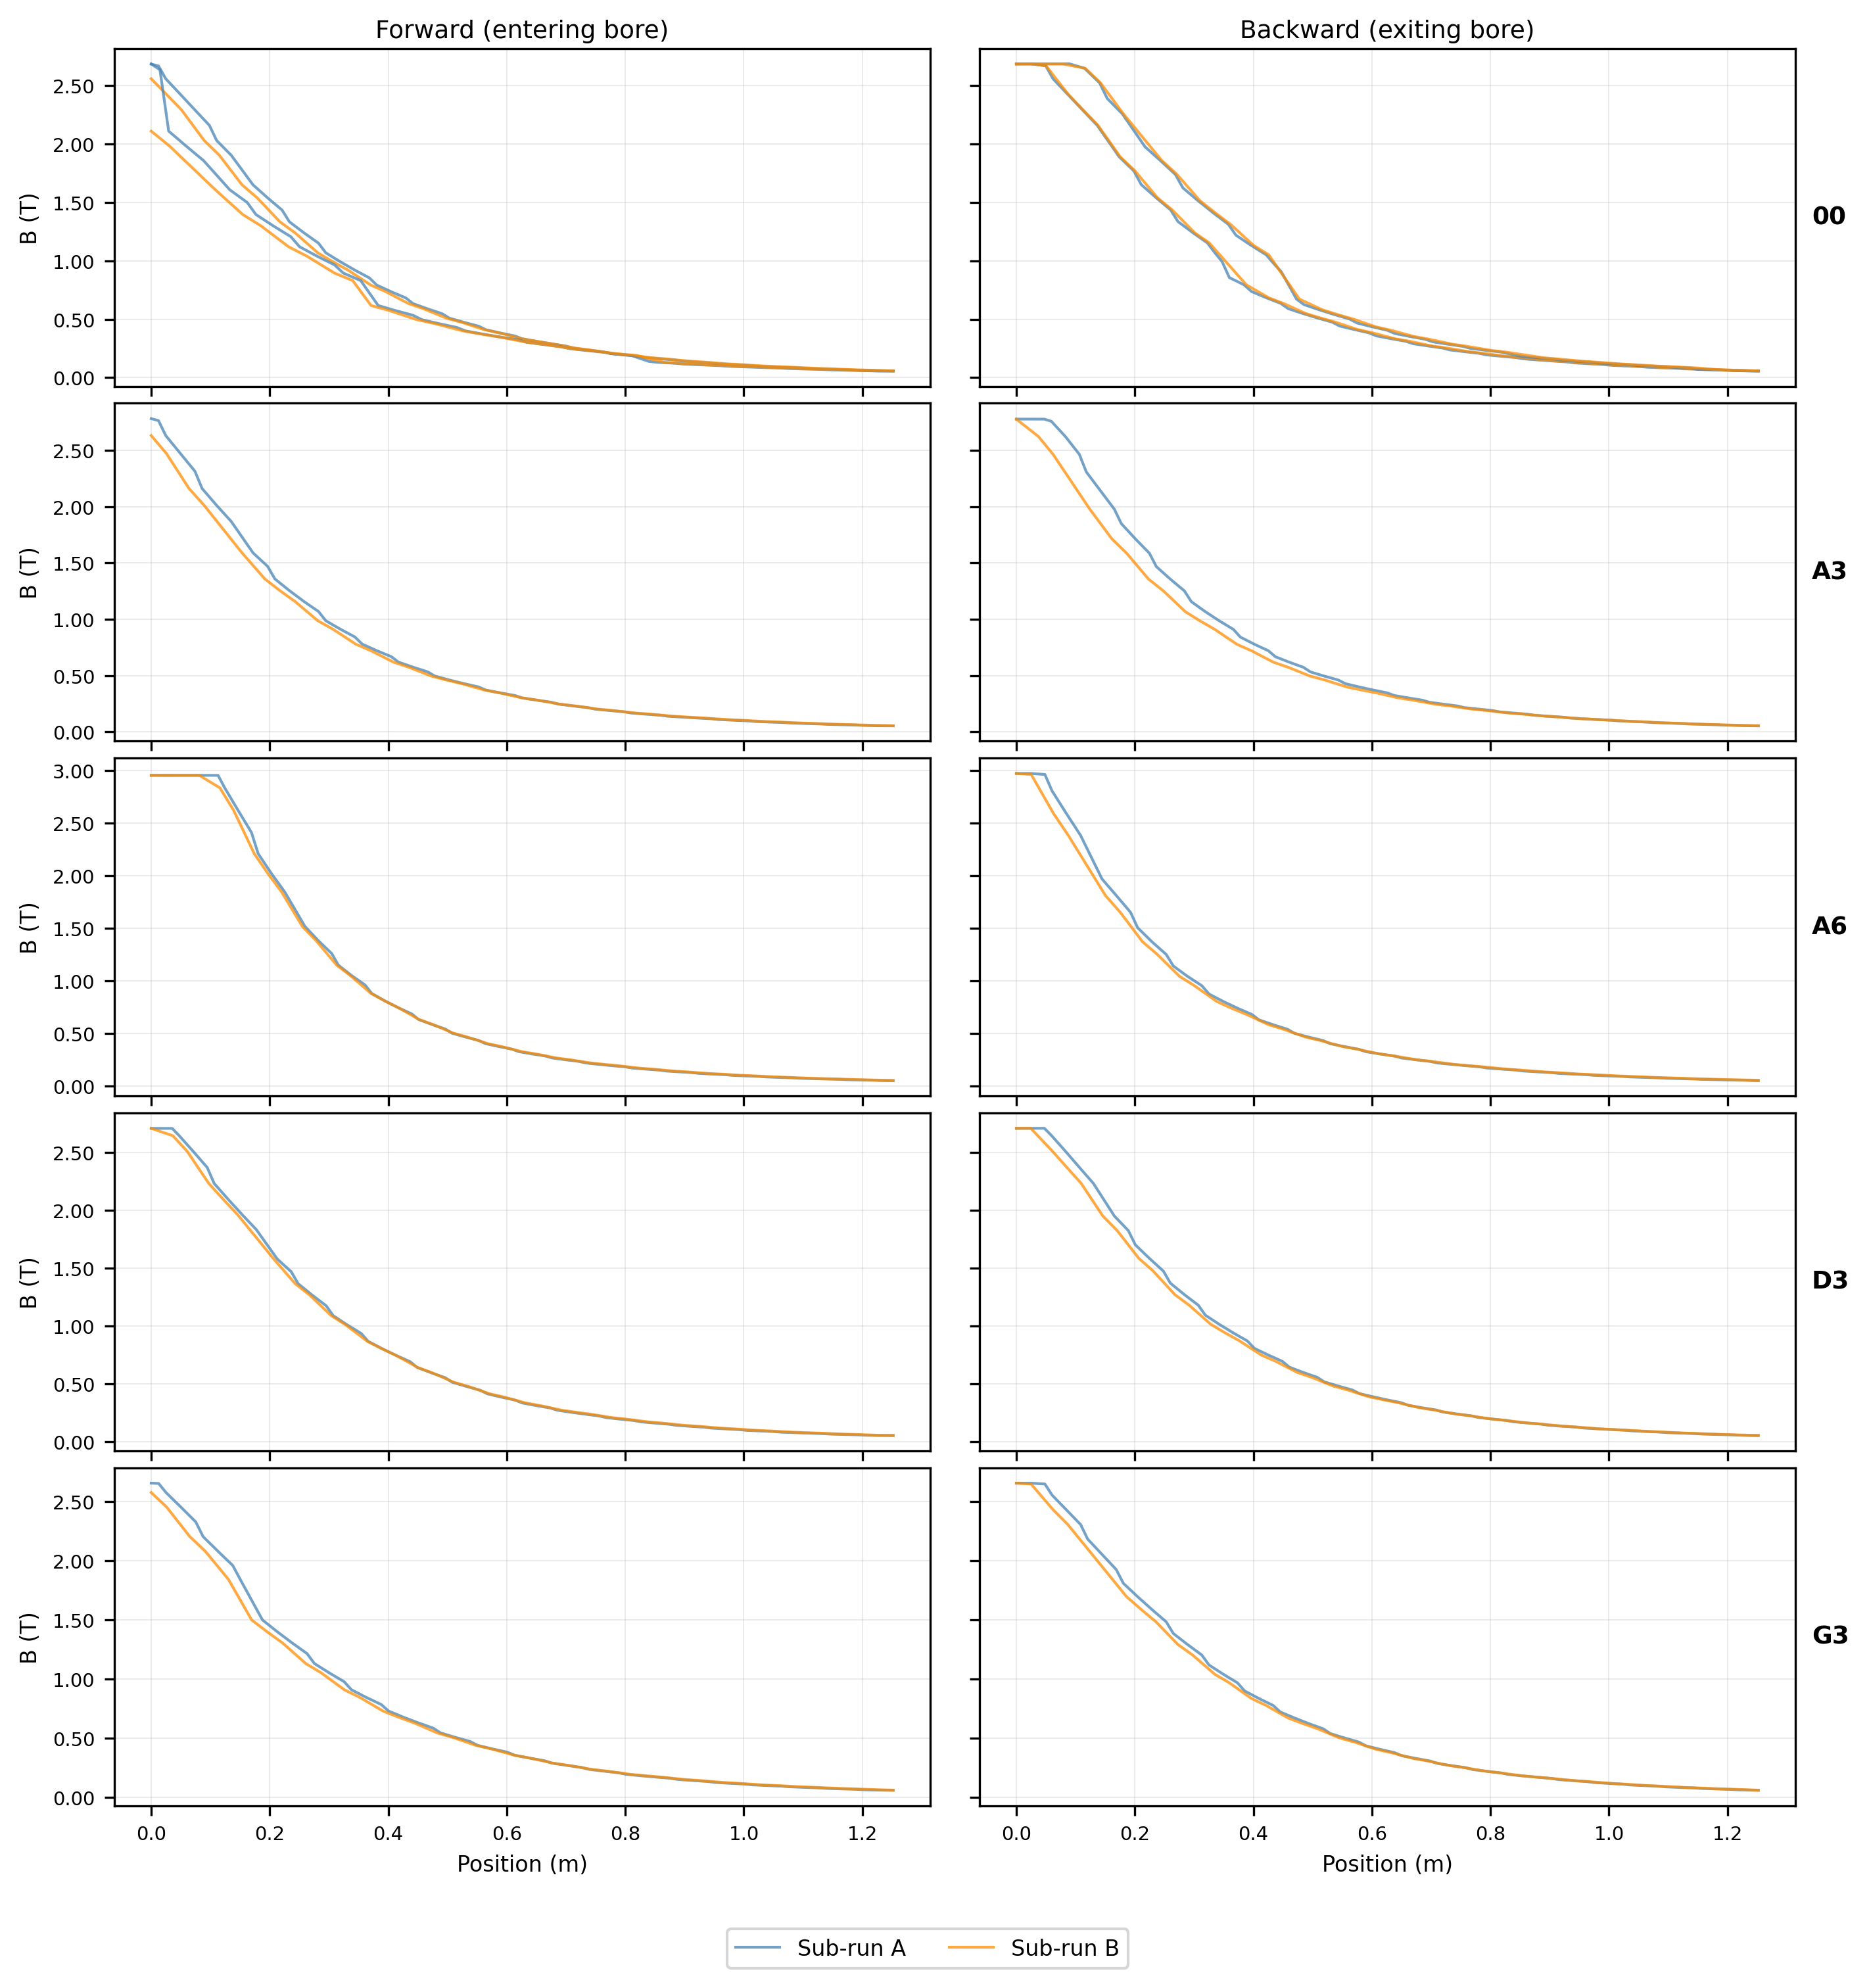
\includegraphics[width=\textwidth]{Assets/allCoords_betterPlots/summary_B.png}
    \caption[$B$ vs position — all coordinates]{%
        Magnetic field $B$ vs position for all five measurement coordinates
        (rows: 00, A3, A6, D3, G3) in forward and backward passes (columns).
        Sub-run A is shown in blue, sub-run B in orange.}
    \label{fig:summary_B}
\end{figure}

% ---------- Figure 2: dB/dz vs Position ----------
\begin{figure}[p]
    \centering
    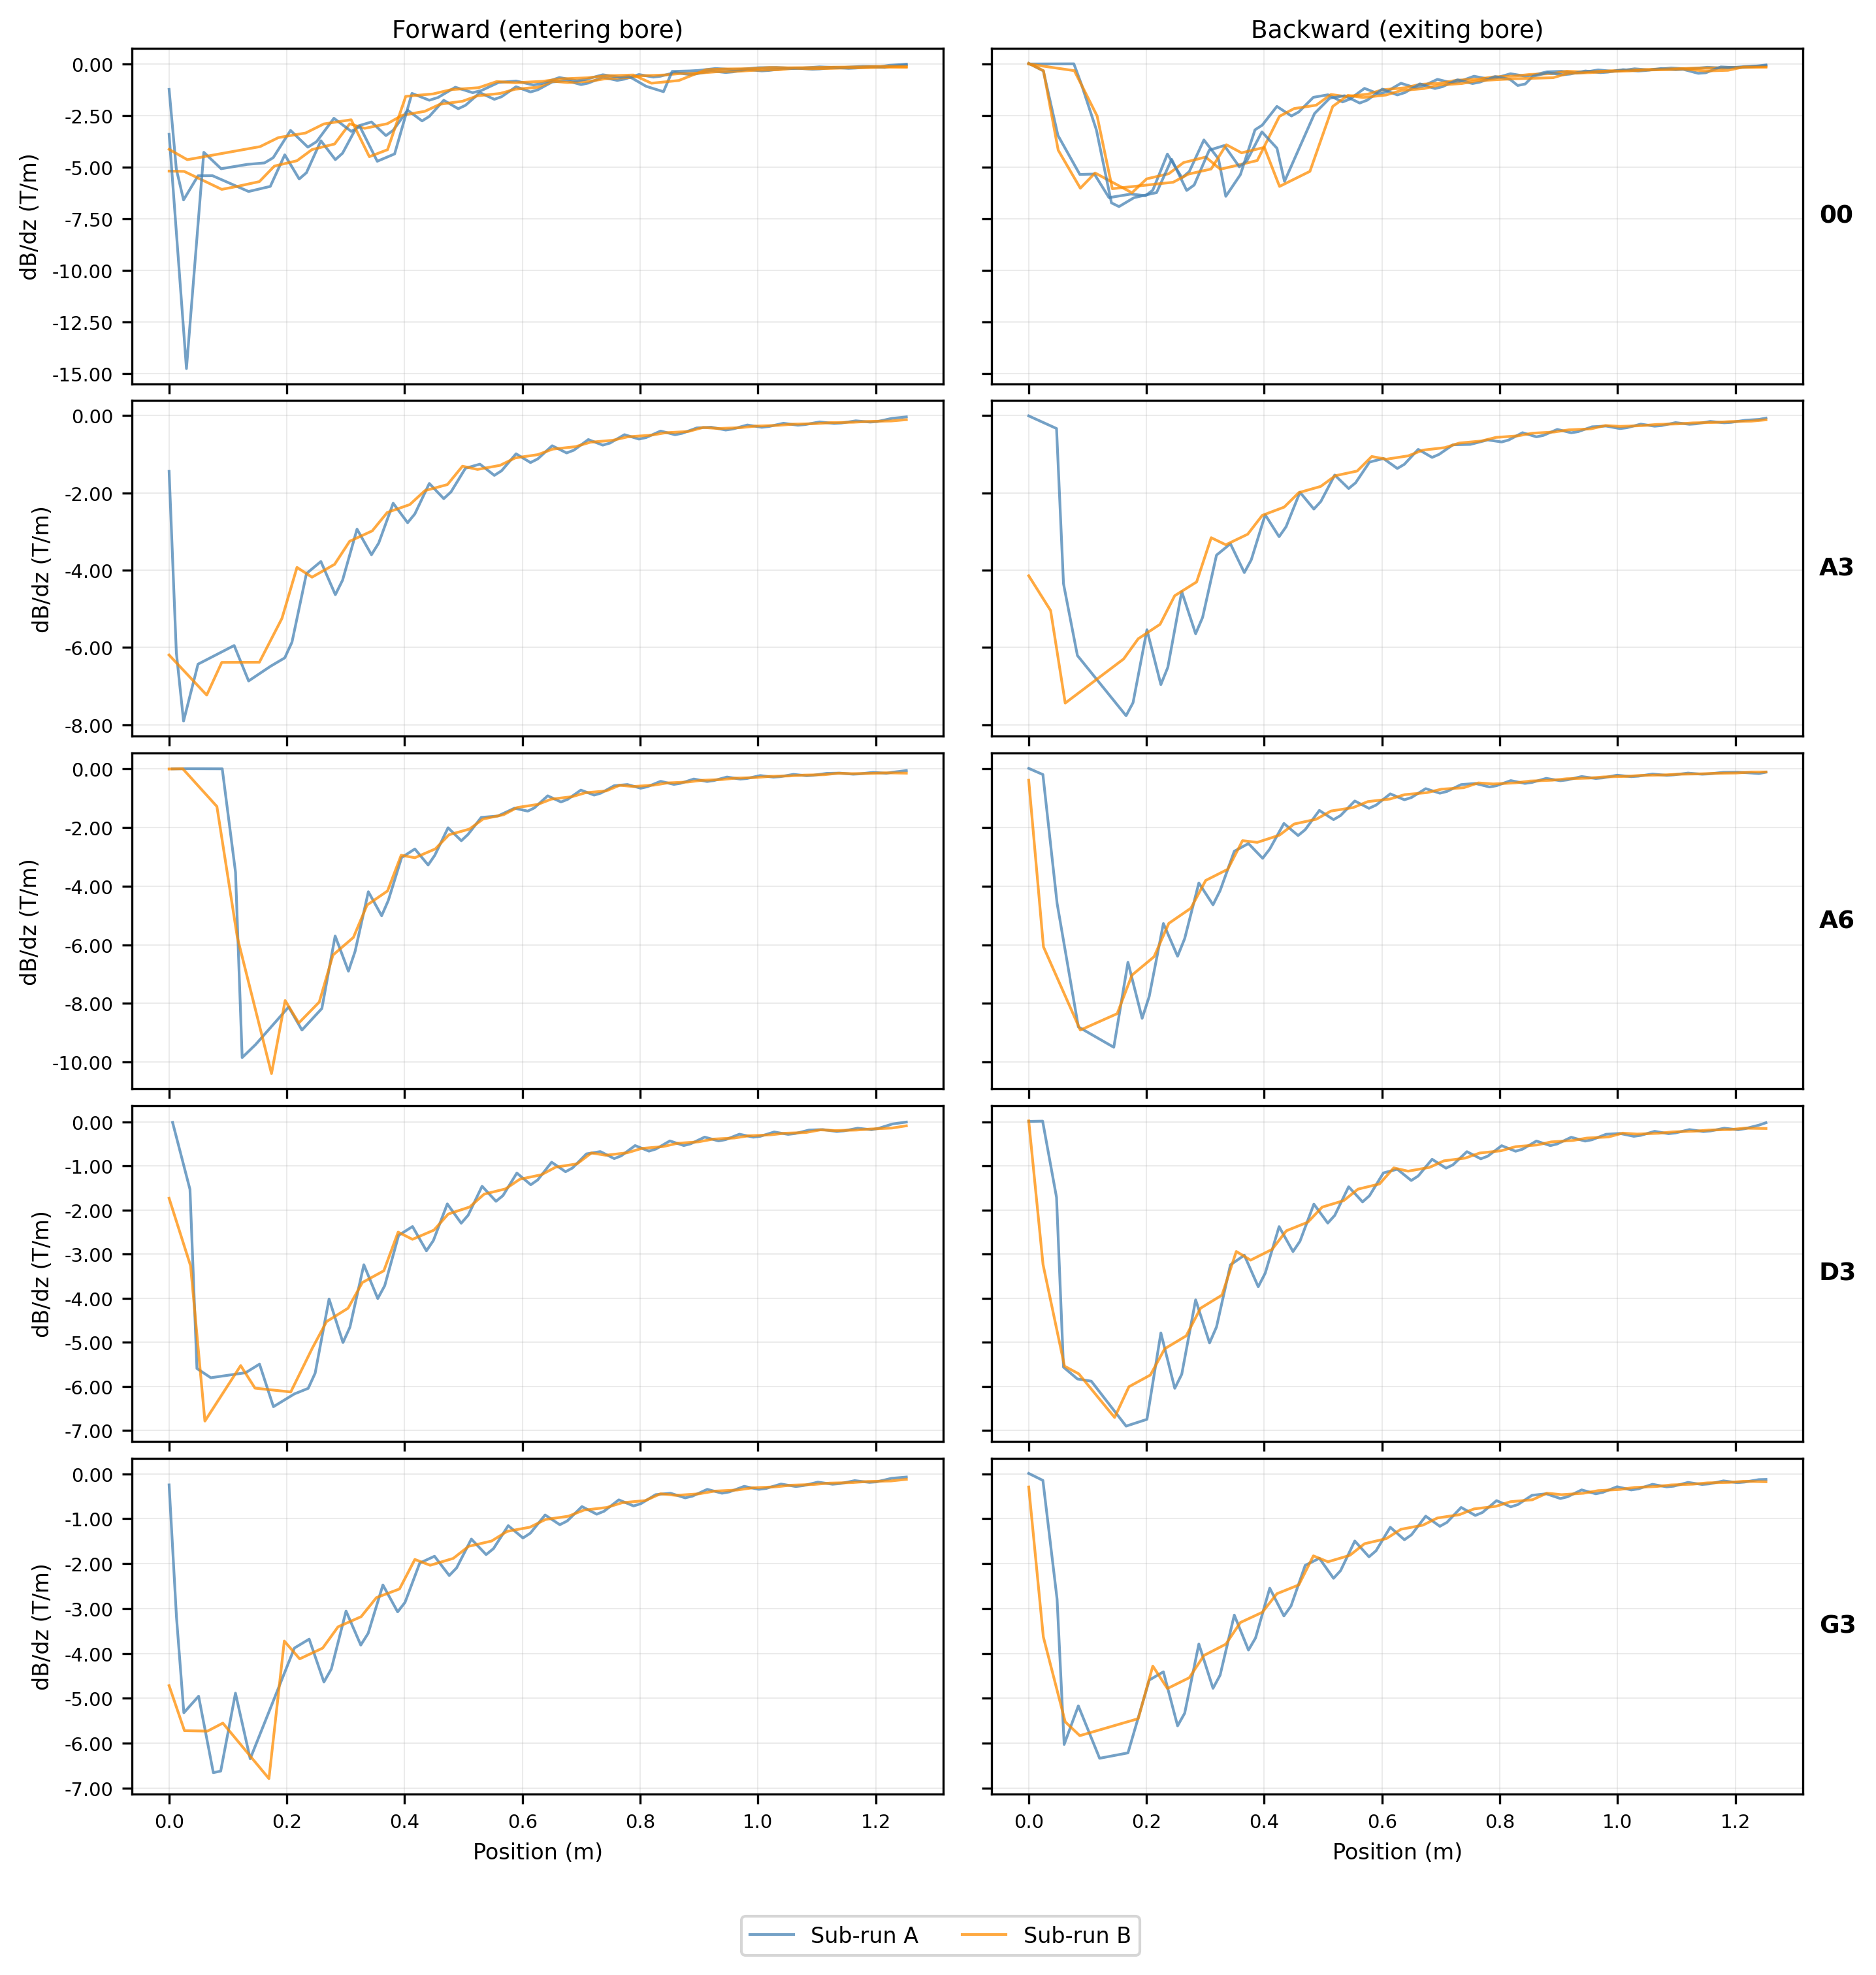
\includegraphics[width=\textwidth]{Assets/allCoords_betterPlots/summary_dBdz.png}
    \caption[$\nabla B$ vs position — all coordinates]{%
        Magnetic field gradient $\mathrm{d}B/\mathrm{d}z$ vs position for all five
        measurement coordinates. Layout as in Fig.~\ref{fig:summary_B}.}
    \label{fig:summary_dBdz}
\end{figure}

% ---------- Figure 3: B·dB/dz vs Position ----------
\begin{figure}[p]
    \centering
    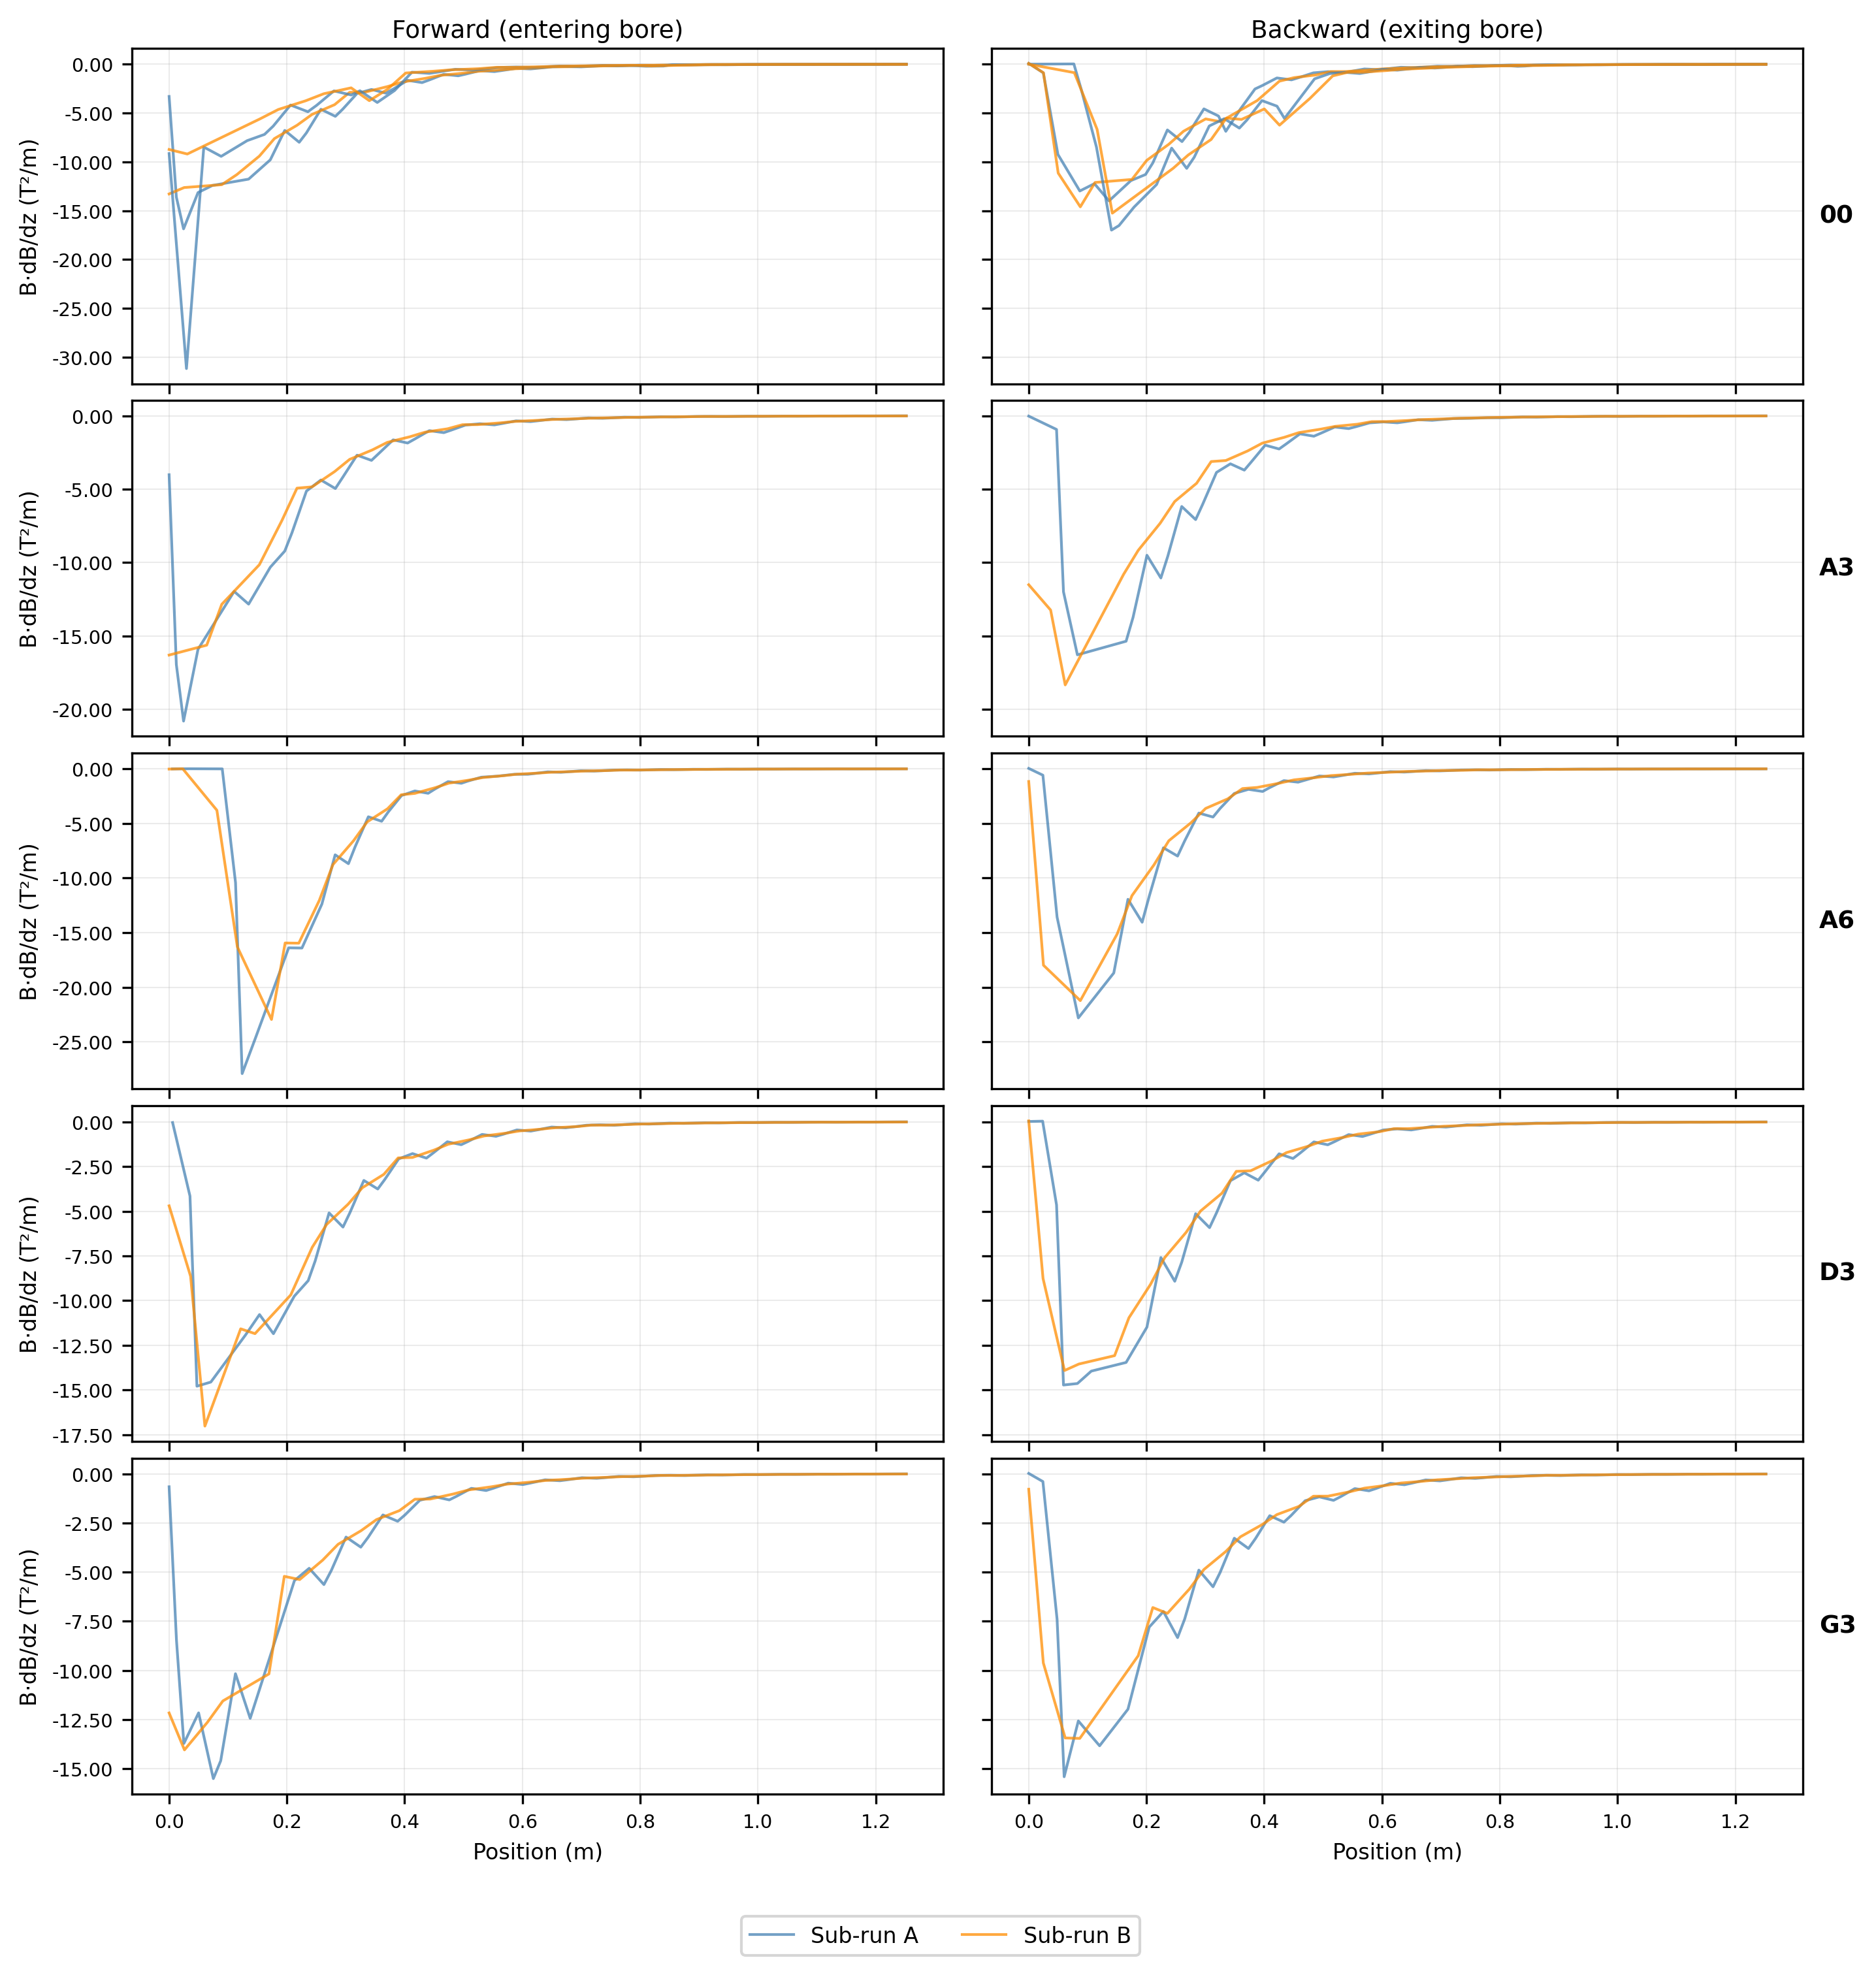
\includegraphics[width=\textwidth]{Assets/allCoords_betterPlots/summary_BgradB.png}
    \caption[$B\nabla B$ vs position — all coordinates]{%
        Product $B\,\mathrm{d}B/\mathrm{d}z$ vs position for all five
        measurement coordinates. Layout as in Fig.~\ref{fig:summary_B}.}
    \label{fig:summary_BgradB}
\end{figure}
